\documentclass{article}
\usepackage{graphicx}
\usepackage{float}
\usepackage{amssymb}
\usepackage{amsmath}
\usepackage{mathrsfs}
\usepackage{bm}
\usepackage{mathtools}
\usepackage{fullpage}
\usepackage{wrapfig}
\usepackage{hyperref}

\newcommand{\norm}[1]{\left\lVert#1\right\rVert}

% \DeclareMathOperator*{\argmin}{arg\,min} % thin space, limits underneath in displays
\DeclareMathOperator*{\argmin}{argmin} % no space, limits underneath in displays
% \DeclareMathOperator{\argmin}{arg\,min} % thin space, limits on side in displays
% \DeclareMathOperator{\argmin}{argmin} % no space, limits on side in displays

\begin{document}

\title{Model Outline}
\author{Octav Dragoi}

\maketitle

\section{Introduction}

The problem is stated as a \textbf{molecule optimization} problem: given one molecule, we wish to come up with another one that improves on certain desirable metrics.

The dataset consists of $N$ pairs of molecules from the set of all molecular graphs $\mathcal{G}$, one being the improved version of the other:
\begin{equation}
    \label{eq:problem_setup}
    D = \{(\mathcal{X}_i, \mathcal{Y}_i) : \mathcal{X}_i, \mathcal{Y}_i\in \mathcal{G}, 1\leq i\leq N\}
\end{equation}

Our model will employ the following components:
\begin{itemize}
    \item A \textbf{Graph Convolutional Network (GCN)}, learning Wasserstein node embeddings in $\mathbb{R}^d, d\in \mathbb{N}$. This takes the shape of a parametric function $G$:
    \[G:\mathcal{G} \rightarrow \mathscr{D}_2({\mathbb{R}^d}),\quad G(\mathcal{X})\in \mathbb{R}^{|\mathcal{X}|\times d} \] 
    where $\mathscr{D}_2({\mathbb{R}^d})$ is the space of all finite point clouds in $\mathbb{R}^d$.
    \item A nonparametric \textbf{tangent space embedding} $\phi = \phi_{Z_0}$ taking a reference point cloud $Z_0\in \mathbb{R}^{N\times d}$. This function, described in \cite{kolouri2020wasserstein}, has the form:
    \[\phi : \mathscr{D}_2({\mathbb{R}^d}) \rightarrow \mathbb{R}^{N\times d}\]
    The main reason why we want to use this function is because it generates workable point cloud embeddings in a \textit{fixed size space}, where we can compute our optimization method. This fixes the problem of variable size embeddings, which are harder to parametrize in a neural network. It also allows the use of pointwise translations for optimizing point clouds with the same number of atoms/points.
    \item A \textbf{Transformer} neural network structure, that learns the molecule improvement within the tangent space.
    \item A \textbf{decoding function} $F\sim G^{-1}$. This function discretizes the optimized tangent vector into a molecular graph $\hat{\mathcal{Y}}$.
\end{itemize}

\section{Training and Inference}

Given the elements described above, we compute the improved model $\hat{\mathcal{Y}}$ as:
\[\hat{\mathcal{Y}} = F(\phi^{-1}(T(\phi(G(\mathcal{X}))))) \]

We set the training loss to be the \textbf{Fused Gromov-Wasserstein}, adding also penalty terms for connectivity and degree constraints.

\begin{equation}
    \label{eq:loss}
    L(\mathcal{X}, \mathcal{Y}) = FGW(\hat{\mathcal{Y}}, \mathcal{Y}) + \lambda_cC(\hat{\mathcal{Y}}) + \lambda_dD(\hat{\mathcal{Y}})
\end{equation}

\begin{figure}[h!t]
    \label{fig:outline}
    \begin{center}
        \includegraphics[page=2,width=\textwidth, trim=0 32cm 0 0 ,clip,angle=0]{images/model_outline_v2.png}
        \caption{Model flow. Compute the predicted graph $\hat{\mathcal{Y}}$, and then use the FGW loss to train the network.}
    \end{center}
\end{figure}

\subsection{Tangent space embedding}

This section discusses a bit more about the embedding function $\phi$, as defined in \cite{kolouri2020wasserstein}. We already exposed the motivation in the introductory part, let us now detail the numerical procedure.

Let $Z_i, |Z_i|=N_i$ be sets of point clouds in $\mathscr{D}_2({\mathbb{R}^d}), 1\leq i\leq M$, and let $Z_0\in \mathscr{D}_2({\mathbb{R}^d}), |Z_0| = N$ be a reference point cloud. Then, we want to view $\phi(Z_i)$ as projections of $Z_i$ on the $\mathscr{D}_2({\mathbb{R}^d})$ manifold's tangent vector space at $Z_0$.

The function $\phi$ is approximated as follows. Let $\pi_i$ be the optimal transport plan between $Z_i$ and $Z_0$, i.e. the solution to the following linear program:
\[\pi_i^* = \argmin_{\pi \in \Pi_i}\sum_{j=1}^N\sum_{k=1}^{N_i}\pi_{jk}\norm{z_j^0 - z_k^i}^2 \]
where $\Pi_i$ is the space of admissible transport plans, i.e.
\[\Pi_i = \left\{\pi\in\mathbb{R}^{N\times N_i}\ \bigg|\ N_i\sum_{j=1}^N\pi_{jk} = N\sum_{k=1}^{N_i}\pi_jk = 1, \forall 1\leq k\leq N_i, 1\leq j\leq N \right\} \]

Then, the Monge map is approximated from the optimal transport plan:
\[F_i = N(\pi_i^*Z_i) \in \mathbb{R}^{N\times d} \]
and the embedding is calculated as:
\[\phi(Z_i) = (F_i-Z_0)/\sqrt{N} \in \mathbb{R}^{N\times d} \]

The function $\phi$ approximates the Wasserstein distance, i.e. $\phi(Z_i) - \phi(Z_0) = W_2(Z_i, Z_0)$ and $\phi(Z_i) - \phi(Z_j) \sim W_2(Z_i, Z_j)$. The quality of this approximation depends on $Z_0$, and therefore $Z_0$ should be picked in an appropriate manner to minimize the error. There is no theoretical bound on the quality of this approximation, though; we will need to check how well it works in practice for our dataset.

As long as the size of the tangent space is larger than the number of nodes of the initial graph, the function $\phi$ is \textbf{fully invertible}; thus, we pick $N$ large enough such that $\phi^{-1}$ is well-defined via simple algebraic matrix inversion.

\subsection{The Transformer}

This section is an implementation of the Transformer paper \cite{DBLP:journals/corr/VaswaniSPUJGKP17}. We believe that the attention mechanism should have a positive influence on the model performance, allowing some nodes to be transformed according to information from other nodes. The relative simplicity and speed of the model makes this model quite fast to train and run.

The initial implementation of this step treats the transfomer as a black box, and modifies the tangent vector embedding $\phi(X) = \phi(G(\mathcal{X}))$ into another tangent vector $T(\phi(X))\in \mathbb{R}^{N\times d}$.

\subsection{$F$ discretizer function}

One can project a tangent vector $y^t\in \mathbb{R}^{N\times d}$ down to a point cloud $Y\in \mathscr{D}_2(\mathbb{R}^d)$. From this embedded point cloud, the model should generate a set of vertices and edges between them.

We want to compute probabilities of node and edge labels, i.e. atom and bond types:
\[P(t(i) = A), P(b(i,j) = A) \]
where $t(i)$ is the type of atom $i$, $b(i,j)$ is the type of bond $j$, and $A$ is some type of atom or bond (with a little bit of notation abuse).

Our model uses feed forward networks to determine labels for the nodes and edges conditioned on the node embeddings. We assume that the node labels depend on the respective node embeddings independently, and edge labels depend on the corresponding pair of node embeddings, so we set up the feed forward networks accordingly.

For bonds, we use a feed forward network taking in a pair of points, and for atoms, just the point embedding:
\[P(b(i,j) = A | y_i, y_j)\quad P(t(i) = A| x_i), \forall i,j \]

% For atoms, we do the following:
% \[P(t(i)|y_i) = \sum_jP(t(i)|y_i,y_j)P(y_j|y_i),\quad \text{where } P(y_j|y_i) = \frac{e^{-\norm{y_i-y_j}/\sigma^2}}{\sum_k e^{-\norm{y_i-y_k}/\sigma^2}}\]

We discretize the logits thus obtained using the Gumbel Softmax.

\subsection{Penalty Terms}

This section describes in detail the penalty terms mentioned in \ref{eq:loss}.

\begin{itemize}
    \item The \textbf{degree constraint} pushes the predicted degree of the nodes to be greater than 1, but smaller than the maximum valency corresponding to the predicted node label. We sample a molecule's node and edge labels using the Gumbel softmax, and then we compute the following expected degree for each node:
    \[E(i) = \sum_{j\neq i}\sum_{B}\left(P(b(i,j) = B)d(B)\right) \]
    where $d(B)$ is the number of edges a bond type implies (None implies 0, single implies 1, double implies 2, etc.)
    We then compute the error term as:
    \[D(\hat{\mathcal{Y}}) = \sum_{i}\left(\min(0, 1 - E(i)) + \min(0, E(i) - \left(\sum_{A} P(t(i) = A)v(A)\right) \right)\] 
    where $v(A)$ is the maximum degree (valency) that an atom of type $A$ can have.
    \item The \textbf{connectivity constraint}, based on the work \cite{2017connectedness}. In short, we sample the adjacency matrix $A$ using the Gumbel softmax, construct the Laplacian matrix $L=\mathbf{diag}(A1) - A$, and then impose the constraint that the matrix
    \[L + \frac{1}{N}11^T  = \mathbf{diag}(A1) - A + \frac{1}{N}11^T\]
    is positive definite. This is equivalent to asking that the graph is connected; proof is in the cited paper. Therefore, we define the following penalty term (for a small $\epsilon > 0$ for numerical stability reasons):
    \[C(\hat{\mathcal{Y}}) = -\log\det\left(L + \left(\frac{1}{N} + \epsilon\right)11^T\right) \]
\end{itemize}

\section{Open Questions}
\begin{itemize}
    \item Setting the parameters for the losses. Can we anneal the weights in such a way that we eventually get 100\% validity rates?
    \item Finding the number of atoms in the predicted set. Right now we cheat and look ahead, taking a barycentric projection from the tangent vector to a point cloud with the appropriate number of atoms.
\end{itemize}

\subsection{Comments and Discussion}

This section is meant for comments and discussion.

\bibliographystyle{ieeetr}
\bibliography{thesisbib}

\end{document}